\documentclass[conference]{IEEEtran}
\usepackage[utf8]{inputenc}
\usepackage[spanish]{babel}
\usepackage{multirow}
\usepackage{amsmath}
\usepackage{float}
\ifCLASSINFOpdf
\usepackage[pdftex]{graphicx}

\else
\fi
\hyphenation{op-tical net-works semi-conduc-tor}

\begin{document}
\title{Desempeño de los MOSFET's y los IGBT's durante su operación en cortocircuito.}
\author{
		\begin{tabular}{c}
			\textbf{Navarro, Facundo Emilio - @63809@electronica.frc.utn.edu.ar} \\ 
			Estudiante de Ingeniería Electrónica - Universidad Tecnológica Nacional - Facultad Regional Córdoba.\\
	\textit{Paper número 9541-30/19}
		\end{tabular}
		}
\maketitle

\begin{abstract}
Tanto los transistores MOSFET's (Metal Oxide Semiconductor Field Effect Transistor) como los IGBT's (Insulated Gate Bipolar Transistor) son dispositivos de potencia controlados por tensión que se utilizan principalmente en conmutación. El primero de ellos fue desarrollado como consecuencia de la búsqueda de una alternativa a las limitaciones de los BJT; mientras que los IGB'Ts combinan algunas de las mejores propiedades de los MOSFET's y de los BJT, ya que ellos son parte de su estructura interna. Este trabajo plantea un análisis del comportamiento de ambos dispositivos bajo la condición de cortocircuito, la cual es muy utilizada en aplicaciones de conmutación, sin que ello pueda significarle un perjuicio.\\

\textit{Abstract}--- As much the MOSFET's transistors (Metal Oxide Semiconductor Field Effect Transistor) like the IGBT's (Insulated Bipolar Gate Transistor) are devices of power controlled by tension that are used mainly in commutation.  First of them it was developed as a result of the search of an alternative to the limitations of the BJT;  whereas the IGBT's combines some of the best properties of the MOSFET's and the BJT, since they are part of their internal structure.  This work raises an analysis of the behavior of both devices under the condition of short circuit, which is very used in applications of commutation, without this can mean a damage to him.
\end{abstract} 

\IEEEpeerreviewmaketitle

\section{Introducción}
\label{sec:intro}
Las propiedades que llevan al MOSFET a ser la elección predilecta a la hora de realizar diseños de potencia son su gran capacidad de conmutar en altas velocidades, el fácil manejo, la capacidad de avalancha y el gran área de operación segura (SOA). Estas ventajas son parcialmente malogradas por sus características de conducción. Además, a medida que la tensión máxima de ruptura aumenta se incrementan las pérdidas en el dispositivo. Los IGBT además de compartir algunas de las propiedades de los MOSFET, poseen características de conducción superiores. Generalmente la velocidad de conmutación del IGBT es inferior a la del MOSFET, pero en los últimos años se han desarrollado nuevas líneas de IGBT que poseen características de conmutación muy cercanas a los MOSFET sin tener que sacrificar las características de mejor conducción. 

\section{MOSFET e IGBT en cortocircuto}
En los MOSFET's los tiempos de conmutación son determinados principalmente por la acción conjunta de sus capacitancias internas e inductancias y la resistencia interna de la fuente de tensión del control de compuerta; el circuito que se utiliza para medir los tiempos de conmutación de un MOSFET puede verse en la Figura \ref{fig:circuit_mosfet}, y los tiempos de conmutación de un MOSFET IRF150 se encuentran representados en ls Figuras \ref{fig:vds_mosfet}, \ref{fig:vgs_mosfet} y \ref{fig:vds_vgs_mosfet}.

\begin{figure}[H]
	\centering
	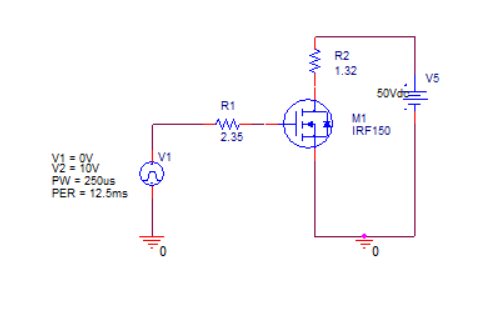
\includegraphics[width=\columnwidth]{imagenes/circuit_mosfet}
	\caption{Circuito para la medición de tiempos de conmutación de un MOSFET}
	\label{fig:circuit_mosfet}
\end{figure}

\begin{figure}[H]
	\centering
	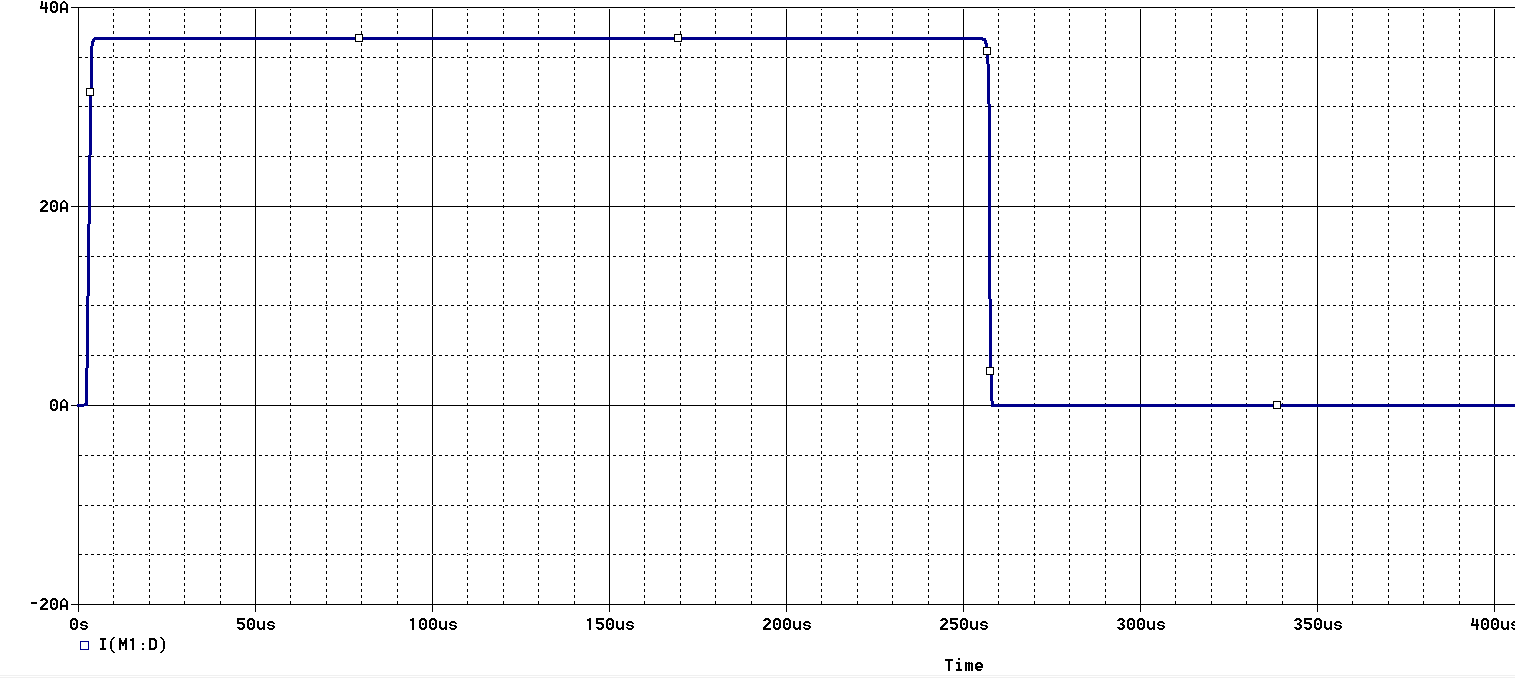
\includegraphics[width=\columnwidth]{imagenes/ic_mosfet}
	\caption{Corriente de colector $I_C$ de un MOSFET}
	\label{fig:ic_mosfet}
\end{figure}

\begin{figure}[H]
	\centering
	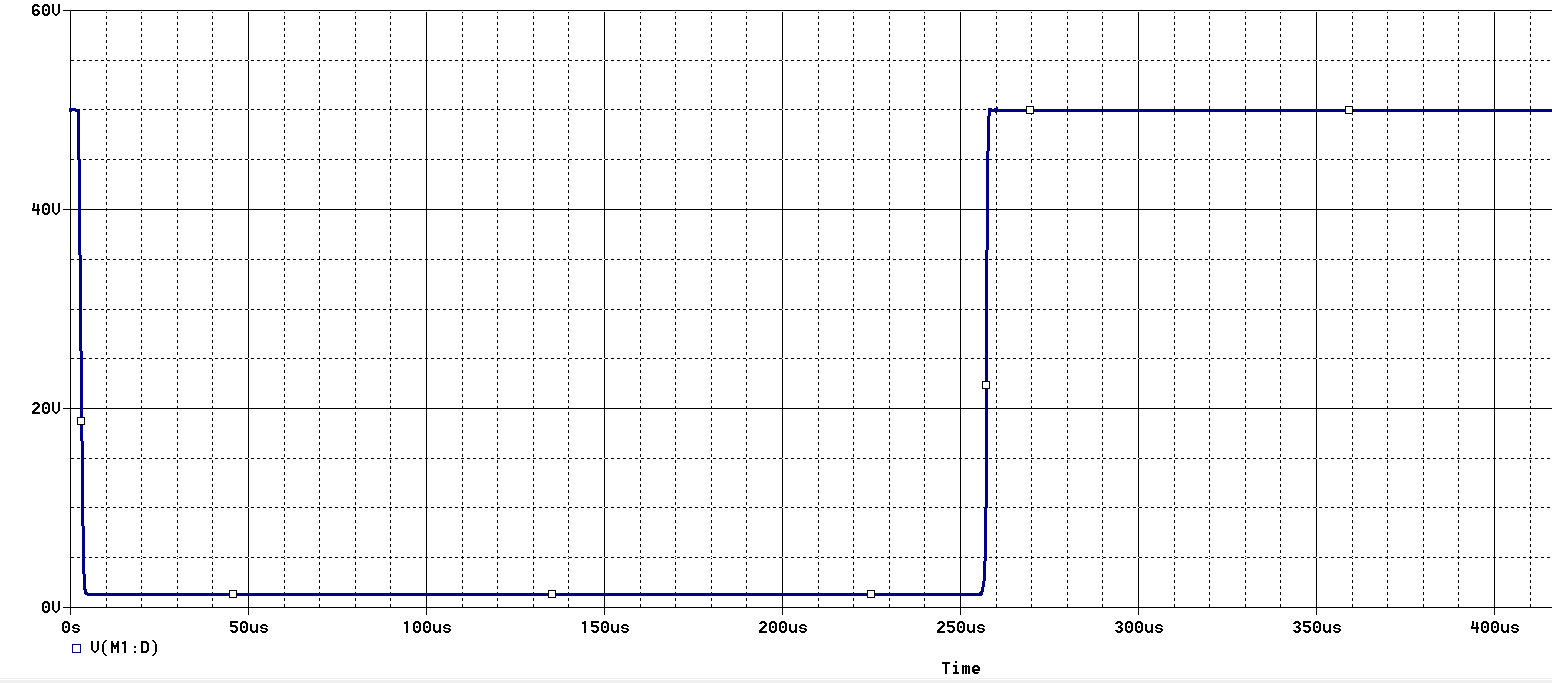
\includegraphics[width=\columnwidth]{imagenes/vds_mosfet}
	\caption{Tensión drenador-surtidor $V_{DS}$ de un MOSFET}
	\label{fig:vds_mosfet}
\end{figure}

\begin{figure}[H]
	\centering
	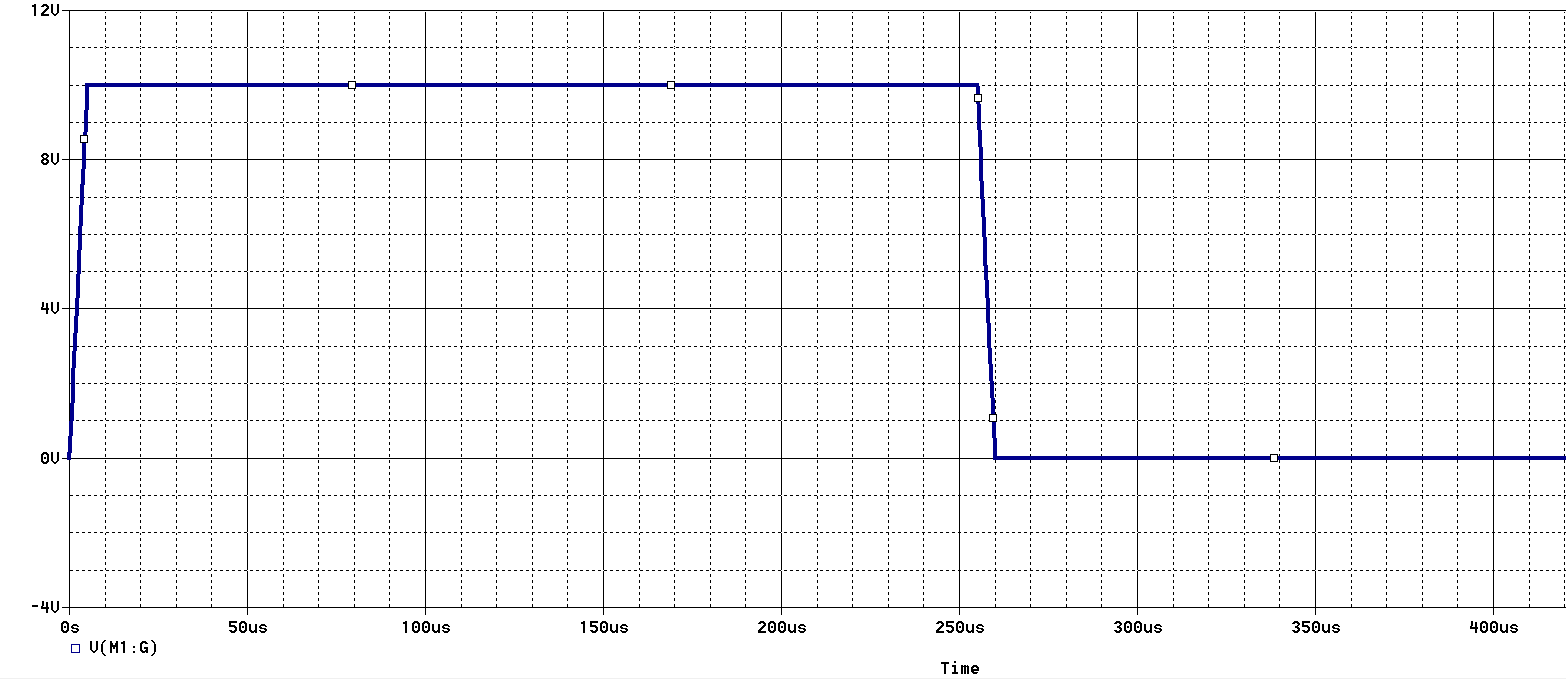
\includegraphics[width=\columnwidth]{imagenes/vgs_mosfet}
	\caption{Tensión gate-surtidor $V_{GS}$ de un MOSFET}
	\label{fig:vgs_mosfet}
\end{figure}

\begin{figure}[H]
	\centering
	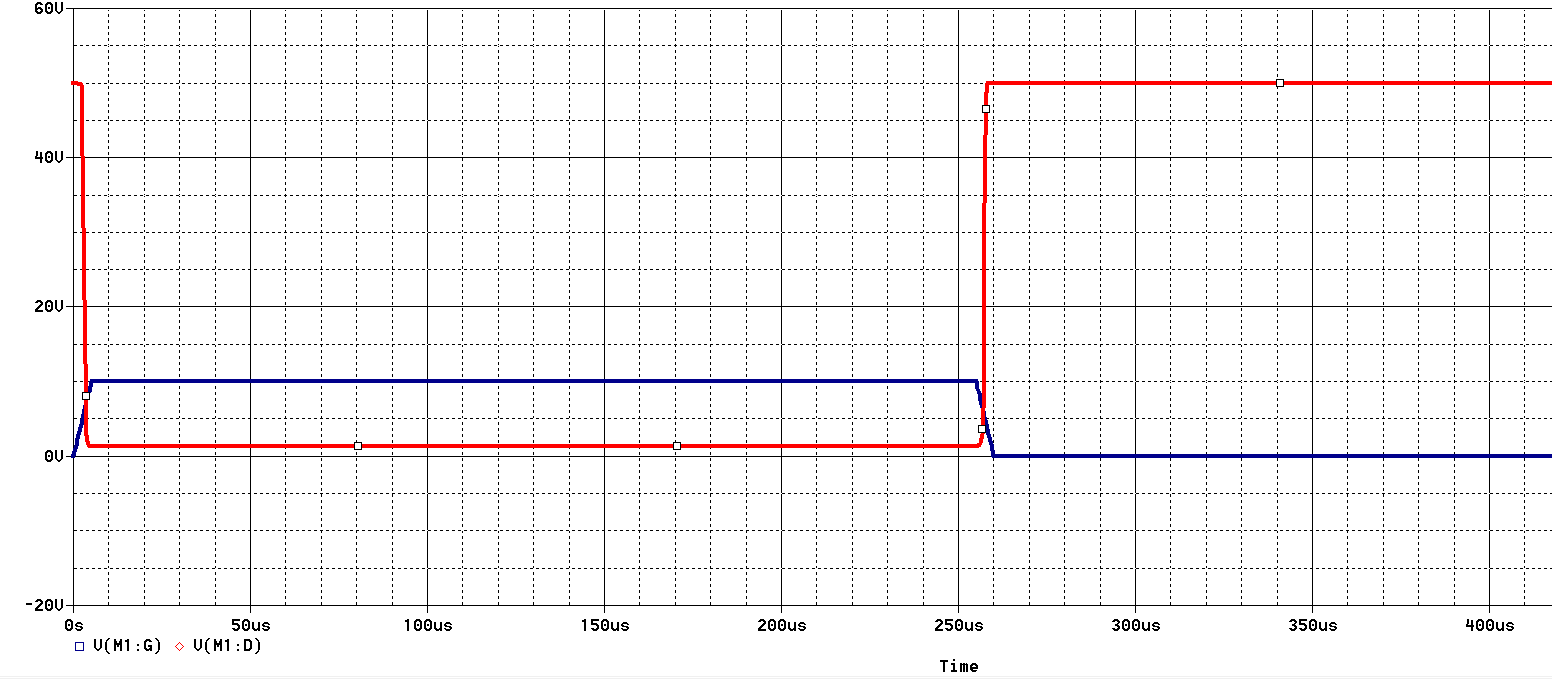
\includegraphics[width=\columnwidth]{imagenes/vds_vgs_mosfet}
\caption{$V_{DS}$ vs $V_{GS}$ de un MOSFET}
	\label{fig:vds_vgs_mosfet}
\end{figure}

Para poder cargar y descargar rápidamente las capacitancias y reducir los transitorios provocados por las inductancias, el generador de tensión del control de compuerta deberá tener una impedancia interna muy baja. La tensión máxima de compuerta no deberá excederse bajo ninguna circunstancia, debido a que esto provoca la falla del dispositivo en forma inmediata. Puede verse en las figuras anteriores que el MOSFET no posee tiempo de almacenamiento, esto se debe a que es un dispositivo de portadores mayoritarios.

Cuando analizamos a los IGBT's, debemos tener en cuenta que sus características de conmutación están relacionadas con la tensión de base y con la corrigen de colector. El circuito que se utiliza en este caso es el de la Figura \ref{fig:circuit_igbt}.

\begin{figure}[H]
	\centering
	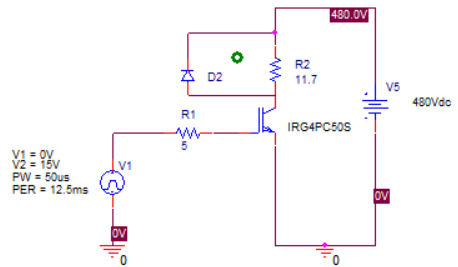
\includegraphics[width=\columnwidth]{imagenes/circuit_igbt}
	\caption{Circuito para la medición de tiempos de conmutación de un IGBT IRGPC50S}
	\label{fig:circuit_igbt}
\end{figure}

Se analizará el caso más crítico, que es cuando el transistor ya está encendido desde antes que se produzca el cortocircuito. En cuanto haya ocurrido el cortocircuito, la corriente de colector se incrementa muy vertiginosamente, esta variación de la corriente está determinada por la tensión de la conexión de continua y por la inductancia del lazo de cortocircuito.

Durante un primer momento el IGBT se encuentra desaturado, la alta variación de la tensión  colector-emisor provoca un desplazamiento de la corriente a través de la capacitancia gate-colector, la cual incrementará la tensión gate-emisor. Esto a su vez causa una corriente pico de corto circuito.
Después de tener completa la fase de desaturación, la corriente de cortocircuito cae hasta su valor estático. Durante este procedimiento, se induce un voltaje sobre la inductancia parásita, el cual aparece como un sobre pico de tensión en el IGBT. 

La fase de cortocircuito estacionario se encuentra seguida del apagado de la corriente de cortocircuito, la cual es conmutada hacia la inductancia de conmutación del circuito, la cual a su vez induce un nuevo sobre pico de tensión en el IGBT.
Estos sobre picos de tensión, inducidos durante el cortocircuito, pueden exceder los valores de operación normal durante algunos momentos. 

En las Figuras \ref{fig:ic_igbt}, \ref{fig:vge_igbt} y \ref{fig:vce_igbt}, pueden verse las gráficas de la corriente de colector, tensión gate-emisor y tensión colector -emisor, respectivamente, de un IGBT.


\begin{figure}[H]
	\centering
	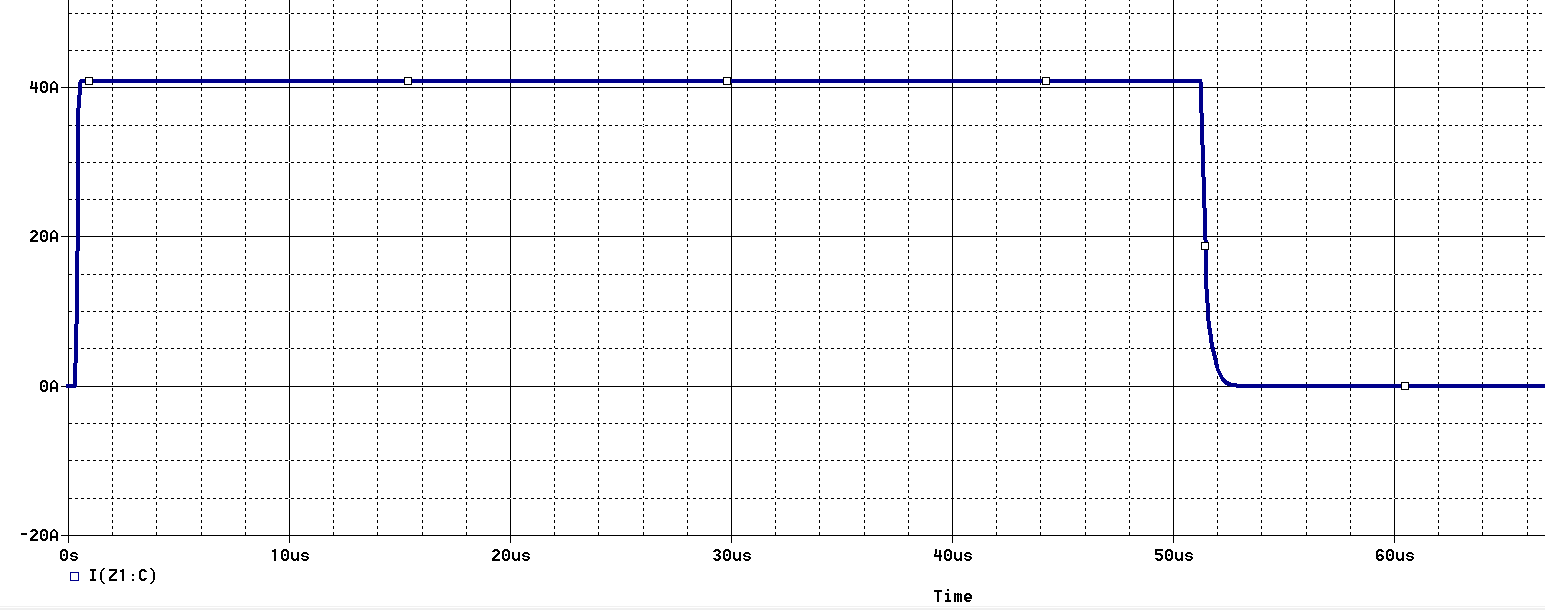
\includegraphics[width=\columnwidth]{imagenes/ic_igbt}
	\caption{Corriente de colector $I_C$ de un IGBT IRGPC50S}
	\label{fig:ic_igbt}
\end{figure}

\begin{figure}[H]
	\centering
	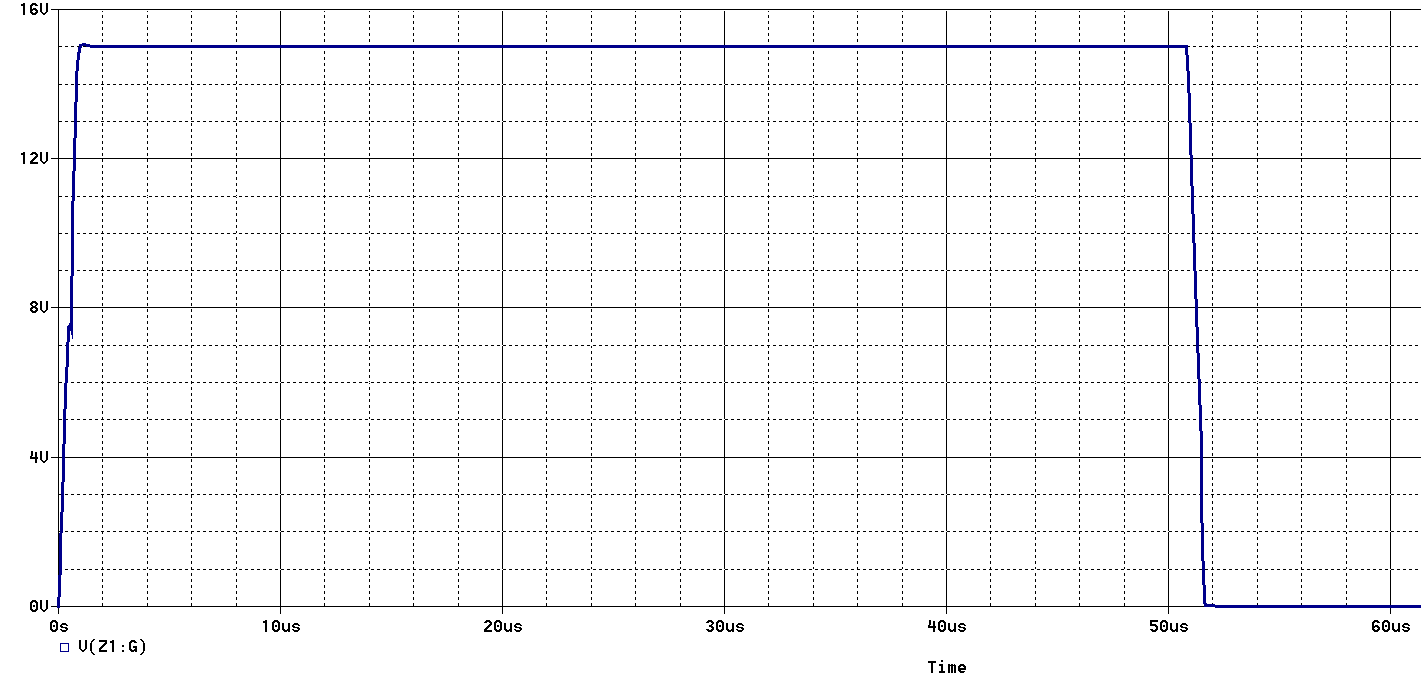
\includegraphics[width=\columnwidth]{imagenes/vge_igbt}
	\caption{Tensión gate-emisor $V_{GE}$ de un IGBT IRGPC50S}
	\label{fig:vge_igbt}
\end{figure}

\begin{figure}[H]
	\centering
	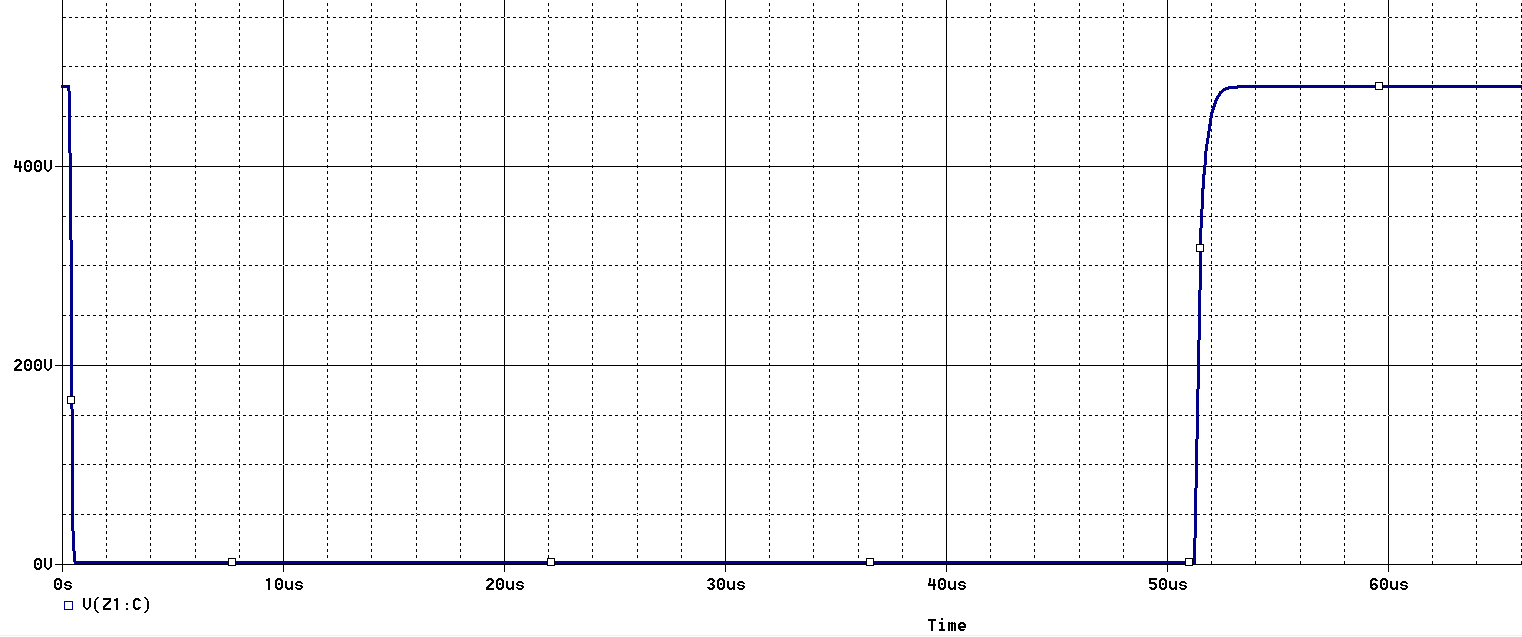
\includegraphics[width=\columnwidth]{imagenes/vce_igbt}
	\caption{Tensión colector-emisor $V_{CE}$ de un IGBT IRGPC50S}
	\label{fig:vce_igbt}
\end{figure}


Los diagramas SOA, como el de la Figura \ref{fig:SOA}, de cortocircuito mostrados en las hojas de datos de los dispositivos muestran los limites seguros para el control de un cortocircuito.
Para garantizar una operación segura deben ser tenidos en cuenta los siguientes límites:
\begin{itemize}
	\item El tiempo entre dos cortocircuitos seguido debe se de, al menos, un segundo.
	\item El cortocircuito debe ser detectado y apagado dentro de un máximo de 10 μs.
	\item El IGBT no debe ser sometido a más de 1000 cortocircuitos durante el tiempo total de operación. 
\end{itemize}

\begin{figure}[H]
	\centering
	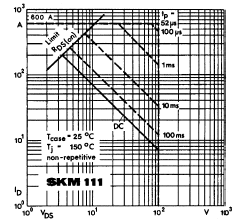
\includegraphics[width=\columnwidth]{imagenes/SOA}
	\caption{Max SOA del MOSFET SKM111}
	\label{fig:SOA}
\end{figure}

Ambos tipos de cortocircuito causan gran disipación de potencia en el transistor, lo cual incrementa la temperatura de juntura. Si el coeficiente de temperatura fuera positivo, la tensión colector emisor se vería favorecida porque habría una reducción de la corriente de colector durante el cortocircuito estacionario.

\section{Conclusiones}
A partir de todo lo analizado se puede comprobar que, tal como se había planteado, es posible trabajar con transistores de potencia tanto MOSFET como IGBT bajo la particular condición de cortocircuito sin que el dispositivo se vea dañado. Es válido recordar que esta condición debe ser aplicada durante períodos de tiempo muy cortos, y de ser repetitivos, el intervalo entre un cortocircuito y el otro debe ser de al menos 1s a fin de no destruir el transistor. Se pudo demostrar que el IGBT, a diferencia de MOSFET que es un dispositivo de portadores mayoritarios, tiene un tiempo de almacenamiento que limita la frecuencia de conmutación que se puede aplicar al circuito, sin embargo compensa esto con sus mejores características de conducción.

\begin{thebibliography}{9}
\bibitem{IEEEhowto:kopka}
Oros, Ramón C. “Dispositivos de Potencia y convertidores de CC y CA” EDUCO. UTN. FRC. Córdoba. Argentina.Edición, Abril 2005. \\ 


\bibitem{IEEEhowto:kopka}
Rashid, Muhammad. “Electrónica de Potencia” Pearson Prentice Hall, México. 2015. \\


\bibitem{IEEEhowto:kopka}
Power electronics handbook : devices, circuits, and applications handbook / edited by Muhammad H. Rashid. – 3rd ed. 2011. \\


\bibitem{IEEEhowto:kopka}
Electrónica de Potencia, Daniel W. Hart; Prentice Hall, 	1995 \\


\bibitem{IEEEhowto:kopka}
Tech notes & Data sheets On Line, Philips Semiconductors.  USA. www.Philips.com \\


\bibitem{IEEEhowto:kopka}
Tech notes & Data sheets On Line, International RectifierInc, www.infineon.com \\


\bibitem{IEEEhowto:kopka}
Tech notes & Data sheets On Line, Semikron Inc,
www.semikron.com \\

\end{thebibliography}

\section{Datos biográficos}

\textbf{Facundo Emilio Navarro}, Nacido en Neuquén el 04/06/1992. Estudiante de Ingeniería en Electrónica, Universidad Tecnológica Nacional, Facultad Regional Córdoba, Argentina. Sus intereses son: Sistemas Embebidos, Procesamiento Digital de Señales, etc.\\

e-mail: 63809@electronica.frc.utn.edu.ar 
\end{document}
